\chapter{Run3における初段ミューオントリガーの性能評価}
実際にRun-3での性能について書く
位置依存性とか大量に

\section{機械学習による Coincidence Window の最適化の効果}
検出器アライメント

チェンバーごとのEfficiency

電荷の依存性



\section{Run-3における初段ミューオントリガー}
Date と MC でeffの比較

\section{Run-3におけるトリガーレート}
Date と MC
\begin{figure}[tb]
  \centering
  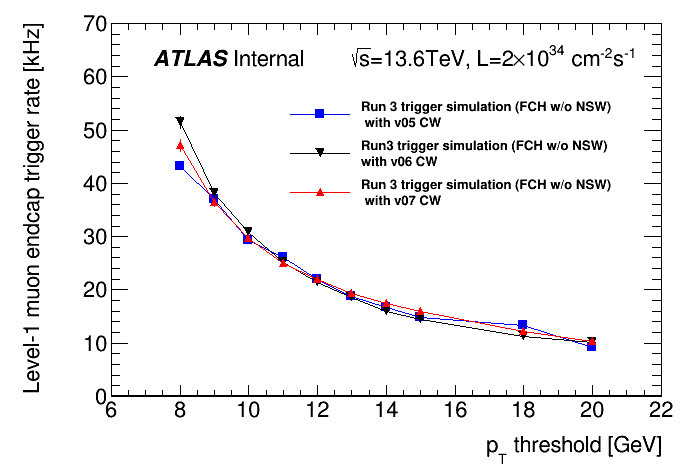
\includegraphics[clip, width=14cm]{fig/5/l1mue_rate_run3.png}
  \caption{Rate}
  \label{fig:fit_def}
\end{figure}


